% Bretthauer: Bis März 2014 Abgabe, 150-200 Seiten max
% Charakter einer Übersicht mit 30-40% Neuheitswert
% Wenn möglich KTI-Professoren zitieren

\chapter{Einleitung}


\zitat{It has often proved true that the dream of yesterday \\
is the hope of today and the reality of tomorrow.}{Robert Goddard}



\section{Bedeutung und Einordnung}
Trotz steigender Benzinpreise ist die Nachfrage nach motorisiertem Individualverkehr ungebrochen \cite{chlond2009mobilitatspanel}. Besonders in den Industrienationen ist seit vielen Jahrzehnten der Pkw als erschwingliches Mobilitätsmittel etabliert, da er seine Insassen bequem und flexibel zum Ziel bringt. Gleichzeitig trübt jedoch das zunehmende Verkehrsaufkommen, vor allem in Ballungsräumen, die Fahrfreude. Denn wenngleich auch der zähfließende Verkehr eine ermüdende Eintönigkeit nach sich zieht, wird dem Fahrer fortwährend eine hohe Konzentrationsfähigkeit abverlangt, sodass er jederzeit in der Lage ist, ein Notmanöver sicher durchzuführen. \\
Gesteigerte Alltagsbelastungen wie Zeitdruck,  Leistungsverdichtung und Informationsflut stellen, insbesondere vor dem Hintergrund einer alternden Gesellschaft \cite{birck2010potenziale}, die Konzentrationsfähigkeit allerdings permanent auf die Probe \cite{NHTSA2006100car}. So wundert es nicht, dass nach 20 Jahren stetig sinkender Opferzahlen in 2011 die Summe der Verkehrstoten auf deutschen Straßen erstmalig wieder anstieg \cite{StatistischesBundesamtDeutschland2012}. Auch heute sterben hierzulande noch durchschnittlich neun Menschen täglich und es werden mehr als 180 schwer verletzt.

Ein hohes Potential, die \mindex{Unfallzahlen} zukünftig weiter zu reduzieren, wird der Unterstützung des Fahrers durch neue elektronische Zusatzeinrichtungen zugesprochen, den modernen Fahrerassistenzsystemen\index{Fahrerassistenzsystem} \cite{handbuchFAS_Winner, maurer2005fahrerassistenzsysteme, eskandarian2012handbook, Bishop2005} (FAS, engl.\ advanced driver assistance systems, ADAS).
So können bereits heute in Serie befindliche %Abstandsreglern und 
Notbremsassistenten\index{Notbremsassistent} überschlägig 
%durch deren automatische Geschwindigkeitsanpassung 
eine %17- bzw.\ \cite{bast07anforderungen}
28-prozentige Reduktion schwerer Unfälle mit Personenschaden vorweisen \cite{gdv2009}.
Bei Lkw wird gar die Wirkung eines Spurhalteassistenten\index{Spurhalteassistent} auf 49 Prozent weniger Unfälle durch Spurverlassen auf Autobahnen beziffert \cite{azt2006}. \\
Ungeachtet der Zahlen tritt beim emotionsgeprägten Autokauf allerdings häufig die Bequemlichkeit in den Vordergrund. Die seit einigen Jahren verfügbaren Komfortsysteme wie Einparkassistent\index{Einparkassistent} und stop-and-go-fähiger Abstandsregeltempomat\index{Abstandsregeltempomat} erfreuen sich immer größerer Beliebtheit und sind längst ein bedeutendes Differenzierungsmerkmal der Fahrzeughersteller geworden \cite{lewandowitz2011markenspezifische}.
Dabei subventioniert, als bemerkenswerter Nebeneffekt, die für die Komfortassistenzsysteme erforderliche Umfeldsensorik langfristig die Verkehrssicherheit\index{Verkehrssicherheit}. Schließlich können die bereits im Fahrzeug befindlichen Radare, Kameras und Laserscanner von den Sicherheitssystemen mit genutzt werden. In ähnlicher Weise leisten auch zukünftige Sicherheitssysteme wiederum ihren Beitrag zur Reduzierung des Fahrzeuggewichts und damit zu einer Effizienzsteigerung, wenn Unfallpräventionssysteme wie der aktive Fußgängerschutz derart verlässlich geworden sind, dass gewichtige passive Sicherheitsmaßnahmen ersetzt werden können. %todo: [NCAP]?

Das aus technischer Sicht hervorstechendste Merkmal der zuvor aufgeführten Sicherheits- und Komfortassistenzsysteme ist der aktive Fahreingriff\index{Fahreingriff}. So wird beim Notbremsassistenten zur Beeinflussung der Fahrzeuglängsbewegung automatisch die Bremse betätigt, falls es aufgrund der Reaktionszeit des Fahrers für eine Warnung zu spät ist. Der Parkassistent wiederum steuert die elektromechanische Lenkung an und zirkelt damit selbständig in enge Parklücken.

Noch sind die serienmäßigen Eingriffe entweder auf niedrige Geschwindigkeiten, geringe Intensitäten oder eine kurze Aktivierungsdauer beschränkt. Die nationalen und internationalen Forschungs- und Entwicklungsaktivitäten bei Fahrzeugherstellern und Automobilzulieferern zeugen allerdings vom Bestreben, langfristig über eine rein unterstützende Assistenzfunktion hinaus zu einer Teil-, Hoch- oder gar Vollautomatisierung \cite{bast2012_rechtsfolgen} zu gehen. Das erfordert allerdings die Aufhebung der zuvor aufgeführten Fahreingriffsbeschränkungen, sodass das volle Dynamikpotential des Fahrzeugs ausgeschöpft werden kann.


Die vorliegende Arbeit behandelt die Optimierung und Realisierung dieser aktiven Fahreingriffe sowie deren Zusammenspiel bei der Umsetzung von Sicherheits- und Komfortfunktionen unterschiedlicher Automatisierungsgrade\index{Automatisierungsgrad}. Im Fokus stehen hierbei ausgewählte mathematische Methoden und Verfahren aus dem Ingenieursbereich (Regelungstechnik\index{Regelungstechnik}) und der Informatik (Robotik\index{Robotik}), die eine hochgradige Relevanz für die behandelte Thematik aufweisen oder gar bereits erfolgreich in Serien- und Prototypensystemen zur Anwendung gekommen sind. Anhand ebendieser Anwendungen aber auch neuer Funktionen wird die methodische Umsetzung der Verfahren praktisch erläutert, wodurch parallel ein tiefer Einblick in die Herausforderungen aktueller Forschungssysteme gegeben wird. 

\section{Entwicklungsstand}
Auch wenn das im Jahr 1940 eingeführte Automatikgetriebe, die seit 1952 verfügbare Servolenkung und der seit 1955 verbaute Bremskraftverstärker bereits in die Fahrzeugquer- und "~längsdynamik eingreifen, so hat sich bis heute der Fahrer so an sie gewöhnt, dass ihre Unterstützung gar nicht mehr als Assistenzfunktion wahrgenommen wird. Neuland wurde 1978 mit der Einführung des Antiblockiersystems\index{Antiblockiersystem} (ABS) betreten, da erstmalig eine elektronische Zusatzeinrichtung zur Anwendung kam, welche Bremseingriffe im Millisekundenbereich ermöglicht. Dank gesteigerter Rechenleistung der sog.\ Steuergeräte sind seither eine ganze Reihe weiterer Assistenzfunktionen verfügbar, die beispielweise durch aktive Fahreingriffe das Durchdrehen der Räder beim Anfahren (Antischlupfregelung\index{Antischlupfregelung}, ASR), das Schleudern des Fahrzeugs beim Ausweichen und in Kurven (Elektronisches Stabilitätsprogramm\index{Elektronisches Stabilitätsprogramm}, ESP), das ungewollte Zurückrollen am Berg (Hill Hold Control) sowie das zu zaghafte Bremsen in Notsituationen (Bremsassistent\index{Bremsassistent})
verhindern. \\
Während sich die zuvor aufgeführten Funktionen mit der Messung \bzw Beobachtung des eigenen Fahrzeugzustands begnügen, gehen Systeme wie der Abstandsregeltempomat\index{Abstandsregeltempomat} (Adaptive Cruise Control, ACC), der Notbremsassistent\index{Notbremsassistent}, der Einparkassistent\index{Einparkassistent} und der aktive Spurhalteassistent\index{Spurhalteassistent} einen Schritt weiter. Mittels Radar-, Kamera- und Ultraschallsensorik macht sich das Fahrzeug ein Bild seiner Umgebung und berechnet entsprechend der umzusetzenden Assistenzfunktion die erforderlichen Fahreingriffe. Um aus Wettbewerbsgründen möglichst früh eine bestimmte Funktion in Serie zu bringen, wurde hierbei in den meisten Fällen kein generelles Regelungskonzept umgesetzt, sondern vielmehr eines, das genau auf ein bestimmtes Standardszenario maßgeschneidert ist. Langfristig geht damit nicht nur ein erhöhter Entwicklungsaufwand der Einzelfunktion einher\footnote{Beispielsweise vergingen nach der Einführung des ersten Parkassistenten viele Jahre bis neben dem Parallel- auch ein Quer-Einparken beherrscht wurde.}, es steigt auch der Integrationsaufwand für das Gesamtfahrzeug enorm, sodass generelle Fahreingriffskonzepte gesucht werden.

Für fahrerlose Forschungssysteme im Umfeld der DARPA Urban Challenge\index{DARPA Urban Challenge}\footnote{Von der Defense Advanced Research Projects Agency ausgetragener Wettkampf zur Förderung der Entwicklung autonomer Fahrzeuge.} stellt sich die Situation ganz anders dar. In 2007 demonstrierten die Finalisten des internationalen Wettkampfes eindrucksvoll, s.\ z.B.\ \cite{urmson2008adu, montemerlo2008junior,bacha2008odin, jfr2008,rauskolb2008caroline,stiller2008probabilistische},  wie souverän sich die stimmigen Gesamtkonzepte ihren Weg durch den, wenn auch stilisierten\footnote{Die Wettkampfregeln klammerten z.B.\ Fußgänger, Fahrrad- oder Motorradfahrer von vornherein aus.}, Vorstadtverkehr suchten. Jede weitgehend zufällig zu Tage tretende Verkehrssituation stellte nur einen Sonderfall für die implementierten Universalkonzepte dar. So manövrierte derselbe Algorithmus, der das Fahrzeug zwischen seinesgleichen parkierte, zielstrebig durch große Parkplatzanlagen oder ließ es zügig am Sackgassenende wenden. Seither sorgen die Weiterentwicklungen der selbstfahrenden Automobile, insbesondere auf öffentlichen Straßen und dank neuer Gesetzgebungen im definierten Rechtsumfeld \cite{CNN2012_legal}, häufig für Schlagzeilen \cite{telegraph2012_google,daimler_faz_2013,Grundhoff2011}.

Weniger davon wachgerüttelt als vielmehr in der ohnehin verfolgten Entwicklungsstrategie bestätigt, arbeitet aktuell die wettbewerbsgeprägte Automobilindustrie fieberhaft daran, die neuen wissenschaftlichen Erkenntnisse aus der Forschung baldmöglichst als kundenwertige Assistenzfunktionen anzubieten. Dabei stellt neben den Kostenaspekten die Anwesenheit des Fahrzeugführers eine große Herausforderung dar. Bei sicherheitskritischen Fahreingriffen will er ja nicht voreilig "`unterstützt"' werden, sodass das Assistenzsystem häufig die Situation sich weiter zuspitzen lassen muss, bevor es eingreifen darf.
Bei den Komfortsystemen hingegen %legt der Fahrer die Messlatte in Bezug auf Verlässlichkeit so hoch, dass 
dient er auf absehbare Zeit als Rückfallebene. Da der Mensch aber nur für kurze Zeiträume seine Aufmerksamkeit automatisierten Abläufen schenken kann, um bei Bedarf korrigierend einzugreifen, muss er mit geeigneten Maßnahmen aktiv in die Regelaufgabe einbezogen werden. 
Zusätzlich erfolgt der Fahreingriff häufig, insbesondere in den Aktivierungsübergängen, in Kooperation mit dem Fahrzeugführer, 
sodass viel Entwicklungs- und Applikationsaufwand betrieben werden muss, bis die Systeme auf breite Fahrerakzeptanz stoßen.


Zusammenfassend kann festgehalten werden, dass die Fahrerassistenz auf dem Weg ist, sich von reinen Fahrdynamik-Regelsystemen hin zur Vollautomation zu entwickeln (s. Abb.\,\ref{fig:Navigation_Fuehrung_Stabilisierung} und für eine detaillierte Prognose bspw.\ \cite{handbookIV_vanArem2012}). Die Primäraufgabe der aktiven Fahreingriffe verlagert sich damit von der Fahrzeugstabilisierungsebene\index{Fahrzeugstabilisierungsebene} hin zur sog.\ Fahrzeugführungsebene\index{Fahrzeugführungsebene}, dem neuen Themenfeld moderner Assistenzsysteme, vgl.\ \cite{handbuchFAS_Donges2012}. Hierbei besteht die große Herausforderung darin, den Fahrzeugführer bedarfsgerecht zu unterstützen, ohne ihn zu bevormunden.

%
\begin{figure}[t]
	\psfrag{1}[cc][cc][1.0][90]{\parbox[c]{7cm}{\begin{center}Regel- \\ systeme \end{center}}}
		\psfrag{2}[cc][cc][1.0][90]{\parbox[c]{7cm}{\begin{center} FAS mit aktiven \\ Fahreingriffen\end{center}}}
	 \psfrag{3}[cc][cc][1.0][90]{\parbox[c]{7cm}{\begin{center} Vollautomatisiertes \\ Fahren \end{center}}}
	%
	\psfrag{a}[cc][cc][1.0]{Navigation}
	\psfrag{b}[cc][cc][1.0]{Führung}
	\psfrag{c}[cc][cc][1.0]{Stabilisierung}
	%
	\psfrag{f}[b][b][1.0]{\parbox[c]{10cm}{\begin{center} Forschung u.\\ Entwicklung \end{center}}}
	%
	\psfrag{k}[cb][cb][1.0]{Sicherheit}
	\psfrag{l}[cb][cb][1.0]{Komfort}
	%
	\psfrag{m}[cc][cc][1.0]{Planungshorizont}
	\psfrag{n}[cc][cc][1.0]{Reaktionsschnelligkeit}
	%
	\psfrag{p}[cc][cc][.8]{($\ldots$)}
	\centering
	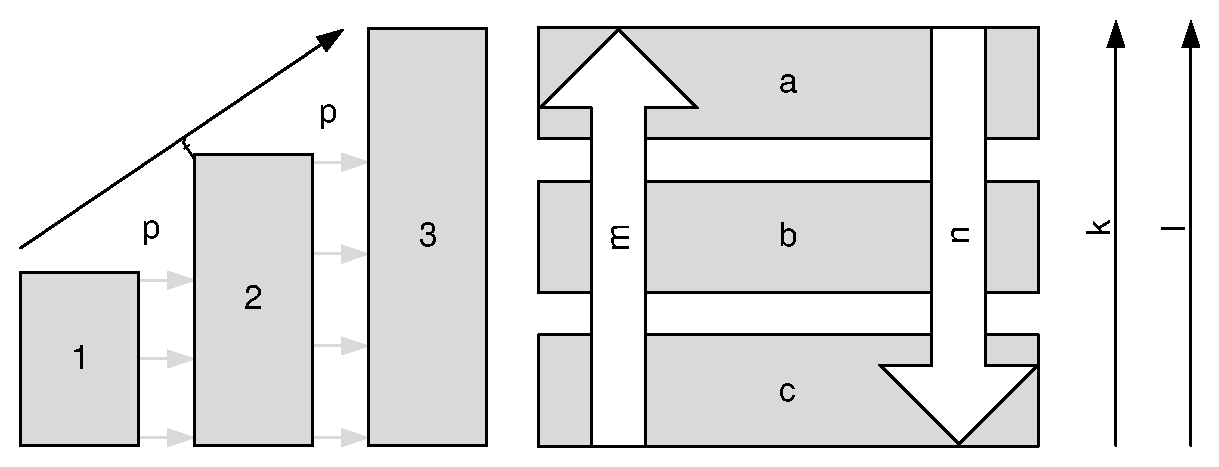
\includegraphics[width=1.0\textwidth]{1_Navigation_Fuehrung_Stabilisierung.eps}
	\caption[Weiterentwicklungstendenzen aus Sicht aktiver Fahreingriffe]{Weiterentwicklungstendenzen aus Sicht aktiver Fahreingriffe dargestellt am Drei-Ebenen-Modell \cite{donges1982aas}}% , vgl.\ \cite{handbuchFAS_Donges2012}}
	\label{fig:Navigation_Fuehrung_Stabilisierung}
\end{figure}

Während die Fahrzeugstabilisierung, vereinfacht gesprochen, von den Ingenieurwissenschaften, und die 
Fahrzeugnavigation (s.\ Abb.\,\ref{fig:Navigation_Fuehrung_Stabilisierung}) 
von der Informatik dominiert wird, überlappen sich beide Disziplinen auf der 
Fahrzeugführungsebene. Grund dafür ist, dass dort das Automobil, ein dynamisches 
System, dessen zielgerichtete Beeinflussung die Aufgabe der Regelungstechnik\index{Regelungstechnik} ist \cite{lunze2005regelungstechnik, unbehauen1989regelungstechnik, foellingeroptimal}, in Interaktion mit seiner Umgebung tritt, welches das Themengebiet der Robotik\index{Robotik} darstellt \cite{Thrun2005,Siciliano2008}. 
Generell befasst sich die Regelungstechnik vor allem mit der Stabilität sowie der Robustheit gegenüber Störungen und Modellfehler eines Systems, beides entscheidende Punkte bei der Funktionsabsicherung von Assistenzsystemen. Die Informatik hingegen widmet sich unter anderem der Lösung stark abstrahierter Probleme mit hoher Komplexität, eine ganz wesentliche Domäne für die "`Intelligenz"' zukünftiger Fahrzeuge \cite{eskandarian2012handbook}. \\
Beide Wissenschaften bedienen sich mathematischer Prinzipien, Methoden und Verfahren, insbesondere aus dem Bereich der Optimierung, die entsprechend der jeweiligen Herangehensweise erfolgreich auf die Fahrzeugführung angewandt wurden. Trotz der thematischen Nähe findet eine direkte Gegenüberstellung, sicherlich erschwert durch die Verwendung unterschiedlicher Fachterminologien, in den seltensten Fällen statt. Gerade aber in einer interdisziplinären Entwicklungsmethodik liegen enorme Chancen, die von Fahrassistenzforschern und "~entwicklern genutzt werden sollten, um modernen Sicherheits- und Komfortsystemen zur Serienreife zu verhelfen.

% Zur Methodik: Optimierung, Graphensuche
% Ing. und Infos kennen oftmals die gegenseitigen Methoden nicht (STabilität: absicherung, Neuplanung, etc.,
% Ingenieure sind stark geprägt durch absicherung: harte Echtzeitanforderungen (roboter darf ruhig mal anhalten um den weg neu zu berechnen.)
% Informatik: Lösungsansätze für komplexe szenarien, Unterschiedliche Begrifflichkeiten) Beispiel mit NMPC und CMU(?)
% Zustandsschätzung der Informatik für best. Probleme überlegen (Patikelfilter, z.B.)
% Unsystematisches Herangehen, Schnittstellen intuitiv gewählt, Aspekte: Modularität, Robustheit
% Ziel: Kombination beider Welten für das Jeweilige Problem
% Planung Informatik: Robotik spezifische intelligente Lösungen
% Planung Regelungstechnik: Stabilität, Störungen, Qualität
% Herausforderung: Freiheitsgrade, Kombinatorik
% Zusammenfassung: Akzeptanz, Kunde, Rechtliche Vorgaben.
%

%Regelungstechnik: 
%- Lehre der Stabilität und Stabilisierung rückgekoppelter dynamischer Systeme
%Rückkopplung ist das wichtigste Grundprinzip der Regelungstechnik
%- Robustheit, Regelgüte, Berücksichtigung oder Kompensation von Störungen, Indentifikation
%
%Mehrebenensteuerung (Lunze I)
%
%Überleitung zu Methoden
%integration bestehender Regelsysteme
%
%Informatik: Millionen von Fahrkombinationen druchspielen

%In Zusammenfassung gilt es, ....

	% Einseitige Bremsung: Spurhalten (Daimler)
% Aktive Lenkeingriffe
	% Unterstützung beim Spurhalten
	% Stauassistenz
% Hinterachslenkung, Torque-Vectoring
% Bei höheren Geschwindigkeiten: Leichte korrigierende Lenkeingriffe zum Spurhalten
%gesteigerten Rechenleistung der Automobilsteuergeräte
% Forschung:
		% 


		
\section{Ziele und Aufgaben}
% Vier Anwendungen: Fzg-Stab: Driften
%										Fzg-Führung + Stab: Anhänger
%										Planung, Führung + Stab: Ausweichen
%            Forschung: NMPC

%	\stich{
% Umfassender Überblick der FAS bzgl. Überschrift, Neuheiten, Konzept zur Bewertung (Bretthauer), Grundsätzliche Motivation für Kapiteleinteilung ohne ins Detail zu gehen \\
%}
Das Hauptziel der vorliegenden Arbeit ist, die Problemstellung aktiver Fahreingriffe derart zu beleuchten, dass Forschungs- oder Entwicklungsteams ein verständlicher Methodenapparat an die Hand gegeben wird, der sie dazu befähigt, neue Sicherheits- und Komfortfunktionen systematisch umzusetzen. Im Einzelnen sind hierzu folgende Teilziele zu erarbeiten: 
\begin{itemize}
	\item Darstellung der Führungs- und Stabilisierungsaufgabe aus Fahrersicht sowie Verdeutlichung der Implikationen für moderne Assistenzsysteme (Kapitel~2)
	\item Übersichtsartige Darstellung der Funktionsweise von Fahrzustands- und Umfelderfassung sowie Aktorik einschließlich ihrer Schnittstellen zum Planungsmodul der Fahreingriffe (Kapitel~2)
%	\item Beschreibung des bestehenden Funktionsumfangs aktueller Fahrerassistenzsysteme der Stabilisierungs- und Führungsebene unter Einbeziehung des abgeleiteten Fahreingriffskonzepts (Kapitel~3 und 4) % Führungsebene: Einparken und Notbremsen
%	\item Vereinheitlichung etablierter Regelungsprinzipien und "~verfahren der automatischen Fahrzeugstabilisierung und Verdeutlichung anhand wichtiger Anwendungsbeispiele aus der Forschungsliteratur (Kapitel~3)
	\item Ableitung eines übergeordneten Fahreingriffskonzepts, welches für typische Assistenzaufgaben das Zusammenspiel von Manöverplanung und "~ausführung einheitlich beschreibt (Kapitel~3)
\item Veranschaulichung mathematischer Methoden zum Nachweis der Durchführbarkeit und Stabilität von Fahrmanövern (Kapitel~3)
	\item Systematisierte Darstellung moderner Manöveroptimierungsmethoden, deren Bewertung hinsichtlich Echtzeitanforderungen und Eignung für verschiedene Einsatzbereiche (Kapitel~4 bis 6) sowie Herausarbeitung von Empfehlungen zu ihrer Kombination (Kapitel~7) 
	%\item Stabilität
	%\item Durchgängige Hinweise auf  und Beispiele zur Implementierung der Methoden und Algorithmen
\end{itemize}
Insbesondere wird durch die hierbei behandelte Materie bei der Beantwortung folgender wichtiger Fragen direkt Hilfestellung gegeben oder auf weiterführende Literatur verwiesen:
\begin{itemize}
%Allgemein: (Kapitel 2)
\item Wann und wie muss ein Sicherheitssystem eingreifen? %Wie wird ein Komfortsystem vorteilhafterweise ein- und ausgeschaltet? 
Wie sieht das Zusammenspiel mit dem Fahrer während des Eingriffs aus? %TTX
\item Wie kann das Fahrzeug über eine seriennahe Sensorik ermitteln, wo es sich befindet oder gerade hinbewegt? Wie ist das Fahrzeugumfeld aus Sicht der Manöverplanung zu repräsentieren? % Odometrie
%\item Was sind die Aufgaben der Planung, was die der Regelung, wie spielen sie zusammen?
%
%Modellierung und Fahrzeugstabilisierung (Kapitel 3)
\item Welche Dynamiken und physikalischen Grenzen des Fahrzeugs einschließlich seiner Aktorik gilt es an welcher Stelle im System zu beachten? Was kann vernachlässigt werden?
\item Welche Störungen und Parameterschwankungen treten in der Praxis auf und wie können sie effektiv kompensiert werden?
%
%Regelung:
\item Wie können Regelziele, "~fehler und "~stellgrößen vorteilhaft definiert werden und wie sind die Schnittstellen zwischen den Einzelsystemen entsprechend zu gestalten?
%\item Welche Regelungsprinzipien und -verfahren haben sich praktisch bewährt?
%\item Vorsteuerung / Regelanteil
%\item Ist die Krümmung eine Störung?
%Planung:
%\item Wie ist das Zusammenspiel mit den restlichen Komponenten?
\item Wie und wo entstehen Rückkopplungen bei der Trajektorienplanung und was muss hierbei beachtet werden?
\item Welche Optimierungskriterien gibt es bei der Planung von Fahreingriffen? Wie können Nebenbedingungen wie Kollisionsfreiheit und fahrphysikalische Grenzen berücksichtigt werden?
%Wie unterscheidet sich die Pfad- von der Trajektorienplanung und wie wirkt sich das auf die Regelung aus?
\end{itemize}

Die Gliederung und die Inhalte der vorliegenden Arbeit orientieren sich am modellprädiktiven Regelkreis\index{Modellprädiktiver Regelkreis} \cite{Lewis_OC}, der vereinfacht in der oberen Hälfte von Abb.\,\ref{fig:Kapiteluebersicht} dargestellt ist. Anhand dessen vermittelt Kapitel~2 die Grundlagen aktiver Fahreingriffe. Während im Anschluss die Stabilität und Robustheit des modellprädiktiven Regelkreises umfassend in Kapitel~3 diskutiert wird, erfolgt die Abhandlung der Fahrzeugführungsaufgabe, also die Trajektorienoptimierung, auf mehrere Kapitel verteilt. Die Gliederung orientiert sich dabei an der klassischen Aufteilung der Methoden zur Lösung dynamischer Optimierungsaufgaben in \emph{Dynamische Programmierung\index{Dynamische Programmierung}, Direkte\index{Direkte Optimierung}} und \emph{Indirekte Optimierungsmethoden\index{Indirekte Optimierung}} (Kapitel~4-6). 
Sie gewinnen bei der Entwicklung von Fahrerassistenzsystemen der Führungsebene weiter an Bedeutung, sodass ihnen der dreifache Kapitelumfang zuteil wird. %Hierbei wird zwischen direkten und indirekten Methoden sowie Methoden der dynamischen Programmierung unterschieden.
Kapitel~7 stellt die wesentlichen Eigenschaften der Optimierungsmethoden gegenüber und gibt ergänzend Empfehlungen zu deren vorteiligen Kombination. Zusätzliche werden dem Neueinsteiger auf dem Gebiet etablierte Handlungshinweisen für die effiziente Erprobung neuer Assistenzfunktionen vermittelt.


\begin{figure}[h]
	\psfrag{a}[cc][cc][1.0]{\parbox[c]{7cm}{\begin{center} Trajektorien- \\ optimierung \end{center}}}
	\psfrag{b}[cc][cc][1.0]{\parbox[c]{7cm}{\begin{center} Unterlagerte \\ Stabilisierung \end{center}}}
	\psfrag{c}[cc][cc][1.0]{\parbox[c]{7cm}{\begin{center} Fahrzeug \end{center}}}
		\psfrag{d}[cc][cc][1.0]{\parbox[c]{7cm}{\begin{center} Messung \\ Zustandsschätzung \end{center}}}
		\psfrag{2}[cc][cc][1.0]{Kap.\,\ref{chap:grundlagen}}
		\psfrag{3}[cc][cc][1.0]{Kap.\,\ref{chap:stabilisierung}}
		%\psfrag{4}[cc][cc][1.0]{Kap.\,\ref{chap:statische_Optimierung}}
		\psfrag{6}[cc][cc][1.0]{Kap.\,\ref{chap:dynamische_Optimierung_direkt}}
		\psfrag{7}[cc][cc][1.0]{Kap.\,\ref{chap:dynamische_Optimierung_indirekt}}
		\psfrag{5}[cc][cc][1.0]{Kap.\,\ref{chap:dynamische_Optimierung_dynamisch}}
		\psfrag{p}[cc][cc][1.0]{\parbox[c]{7cm}{\begin{center} Direkte \\ Methoden \end{center}}}
		\psfrag{q}[cc][cc][1.0]{\parbox[c]{7cm}{\begin{center} Indirekte \\ Methoden \end{center}}}
		\psfrag{o}[cc][cc][1.0]{\parbox[c]{7cm}{\begin{center} Dynamische \\ Programmierung \end{center}}}
		%
		\psfrag{m}[cc][cc][1.0]{\parbox[c]{7cm}{\begin{center} Dynamische \\ Optimierung \end{center}}}
		%\psfrag{n}[cc][cc][1.0]{\parbox[c]{7cm}{\begin{center} Statische \\ Optimierung \end{center}}}
	\centering
  	%\includegraphics[width=1\textwidth,clip, trim = 0cm 0cm 0cm 0cm]
	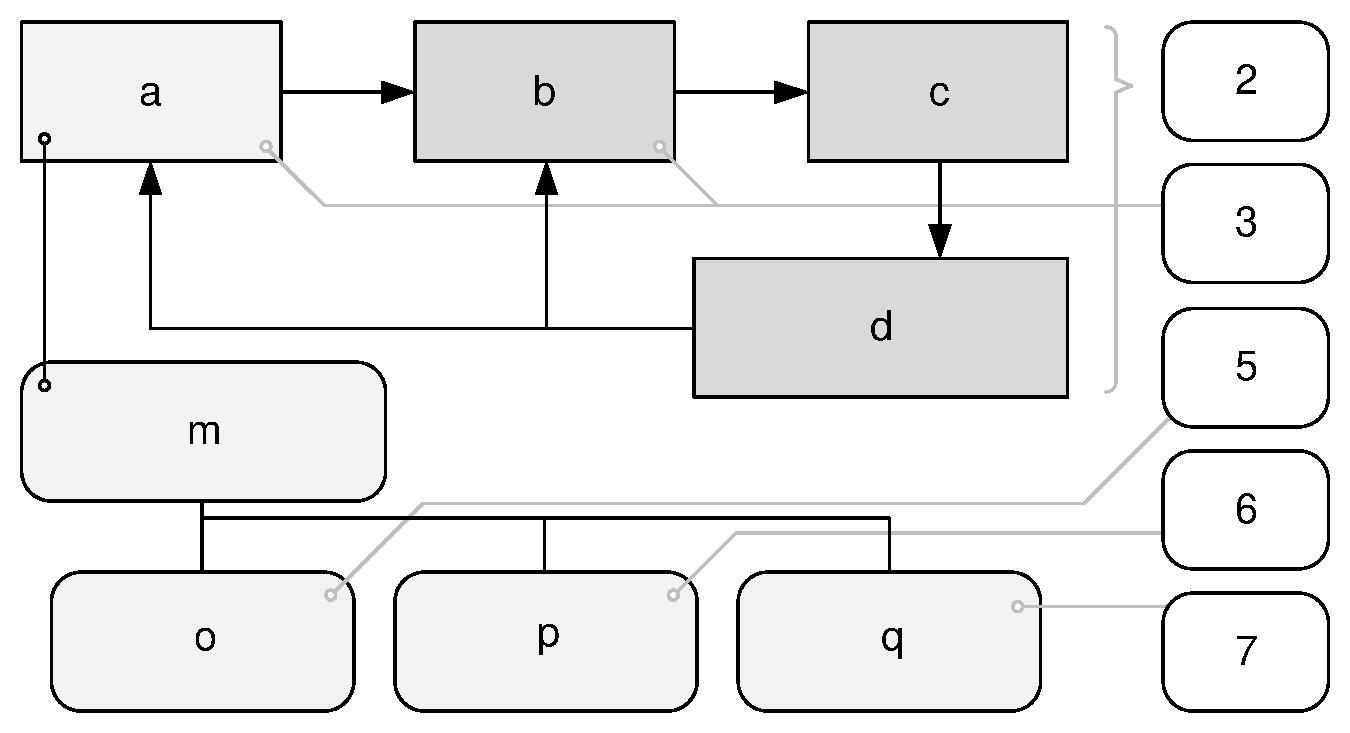
\includegraphics[width=1.0\textwidth]{1_Kapiteluebersicht.eps}
	\caption{Gliederung der Arbeit dargestellt am modellprädiktiven Regelkreis}
	\label{fig:Kapiteluebersicht}%
\end{figure}

Damit gibt die vorliegende Arbeit erstmalig einen systematisierten Überblick zu Methoden, Systemkomponenten sowie deren Verknüpfungen zu Sicherheits- und Komfortsystemen mit aktiven Fahreingriffen. Bei der pädagogischen Themenaufbereitung orientiert sie sich insgesamt an Studenten, Einsteigern und Fortgeschrittenen. Insbesondere bei der Definition der Aufgabenverteilung und dem Zusammenspiel zwischen permanenter Manöveroptimierung und unterlagerter Fahrzeugstabilisierung wird wissenschaftliches Neuland betreten. Darüber hinaus werden neue Algorithmen der Fahrzeugstabilisierungs- und der Fahrzeugführungsebene detailliert hergeleitet und anhand realer Fahrversuche und Simulationen validiert, sodass zusätzlich ein tiefer Einblick in den Kern neuer Assistenzsysteme gegeben wird.

\cleardoublepage

%TODO: % Warnende Systeme haben den Nachteil, dass die Reaktionszeit vom Fahrer hinzukommt. Außerdem muss er dann genau wissen, was er zu tun hat.

% Ideal: je näher in der zukunft desto stärker zählt die physik, je weiter weg, desto eher zähen die Verkehrsregeln und die interaktion

% STVO: gibt heuristiken vor, sodass ics verhindert werdn.

% Selbst wenn die Zukunft genau bekannt ist, ist eine TP, die garantien ausspricht nicht trivial.


%10 Thesen:
%
%Die Anwendungskapitel sind einheitlich aufgebaut, um deren Durcharbeitung zu vereinfachen.
%
%Die Algorithmen der Anwendungsbeispiele sind wissenschaftlich neu.
%
%Alle Anwendungsbeispiele (Kap. 3-7) sind praxiserprobt.
%
%Der Leser erhält sowohl theoretische als auch praktische Aspekte der.
%
%Best-practice mit Hinweisen auf häufig gemachte, zeitraubende Fehler.
%
%Ausgiebige Literaturangaben erleichtern das Folgestudium
	%
	%Sammelwerk aus Methoden der L- und NL-Regelung, welche sich im Automotive-Bereich in der PRAXIS bewährt haben. Dadurch hat der Student die Gewissheit, dass die die Praxistauglichkeit gegeben ist.



	
	%Neben dem obligatorischen ersten und letzten Kapitel, stellen die
%Anwendungskapitel 4, 5, 6 und 7 den Kern der Arbeit dar und sind
%"wissenschaftlich neu". Diese sind so gewählt, dass die beschriebenen
%Funktionen auf aktiven Lenkeingriffen beruhen und die
%Assistenzspektren "Niedriger Unterstützungsgrad" bis "Hoher
%Unterstützungsgrad" sowie "Niedrige Querdynamik" bis "hohe
%Querdynamik" abdecken.
%
%Kapitel 4 stellt die Erweiterung des automatischen Einparkens auf
%Fahrzeuge mit Anhänger dar. Es werden zwei Regler entworfen, die es
%ermöglichen, entweder nur den Knickwinkel des Anhängers zu
%stabilisieren, was die permanente Anpassung der Sollvorgabe vom Fahrer
%erfordert, oder dass das Fahrzeug eigenständig einen geometrischen
%Pfad stabilisiert (z.B. Einparken). Hierzu bereite ich gerade einen
%at-Beitrag vor.
%
%Kapitel 5 demonstriert, wie mit Hilfe der Lenkung (und nicht wie
%herkömmlich mit Einzelradbremsungen) ein schleuderndes Fahrzeug
%abgefangen oder (für Fahrertrainingszwecke) absichtlich unter
%Zuhilfenahme des Motormoments im Driften gehalten werden kann. Im
%Unterschied zu bisherigen Arbeiten ist das Besondere hierbei, dass der
%Regler als Parameter ausschließlich die Lenkübersetzung braucht
%(robuster Sliding-mode-Regler) und nur die Seriengierrate rückführt.
%Eine Veröffentlichung ist in Arbeit.
%
%Kapitel 6 stellt eine algorithmisch unbedeutende, für die Praxis aber
%umso wichtigere Funktion dar, welche Kollisionen im Seitenbereich
%(Spurwechsel mit Fahrzeug im Toten Winkel) verhindert. Hierzu wird,
%wie auch im nächsten Kapitel, auf die Fahrzeugumfeldsensorik
%zurückgegriffen.
%
%Kapitel 7 wird den größten Umfang haben, da hier mein
%Forschungsschwerpunkt liegt. Ich beschränke mich auf zwei Ansätze der
%Optimalsteuerung. Der indirekte Ansatz zeichnet sich durch schwer zu
%unterbietende Rechenzeiten aus, sodass dieser auf aktuellen
%Steuergeräten problemlos umgesetzt werden.
%Bei Kombination mit Bremsmanövern bekommen die fahrphysikalischen
%Restriktionen und die Fahrzeug-Nichtlinearitäten ein höheres Gewicht,
%sodass diesen mit einem direkten Ansatz, der nichtlinearen
%modellprädiktiven Regelung, begegnet wird. Für letzteres ist das Paper
%auf der CDC angenommen worden.
%
%Da sich die verwendeten Methoden auf andere Assistenzsysteme anwenden
%lassen, die aus Platzgründen nicht beschrieben sind (und mit denen ich
%mich, bzw. mein Doktorand, auch erst in Zukunft beschäftigen werde),
%und um die Anwendungskapitel leserlich zu gestalten, habe ich die
%Regelungsmethoden in Kapitel 3 vorverlagert.
%
%Das davor befindliche Kapitel 2 beinhaltet schließlich neben den von
%mir angesammelten "best-practice" Erfahrungen, weitere wertvolle
%Grundlagen (auf die im Anschluss zurückgegriffen wird), sodass der
%Leser einen guten Überblick über alle wichtigen Begriffe der Hartware-
%und Softewarekomponenten sowie deren Bedeutung für die
%Fahrerassistenzforschung bekommt.
%


	
	
%Mit Achsen:
%----------------------------- niedrige Fahrdynamik ------------- hohe Fahrdynamik --
%hoher     Unterstützungsgrad:	[1 Rangierassistenz]  						 [2 Driftassistenz]
%niedriger Unterstützungsgrad: [3 LCA]               						 [4 Kombinierte Brems-Ausweich-Assistenz/Integrierte Kollisionsvermeidung]           
%hoher Unterstützungsgrad:     permanent
%niedriger Unterstützungsgrad: kurzzeitig (keine Aussage über Wirksamkeit!), haptische Untersützung, kein Anspruch auf eigenständiges Lenken.
%
%niedrige Fahrdynamik/Querdynamik: 				kaum Querbeschleunigung oder Schräglaufwinkel
%hohe Fahrdynamik/Querdynamik: 						erhebliche Querbeschl. oder Schräglaufwinkel
%
%
									%
%
%Mit Beschriftung							
%----------------------------- Komfort ---------------- Sicherheit --
%Lenken alleine:			        [1 Rangierassistenz]  		[3 LCA, falls kein Bremseingriff]
%Kombination mit Gas/Bremse: [2 Driftassistenz]        [4 Kombinierte Brems-Ausweich-Assistenz/Integrierte Kollisionsvermeidung
